\begin{comment}

En un programa escrito en lenguaje máquina, el control de
flujo se lleva a cabo, esencialmente, a través de una
instrucción {\tt goto}. Según el relato de
\citet[p. 264]{1974_Knuth}, el Dr. Eiichi Gotō
%
% Para cambiar de tipo de letra en algún fragmento:
%
({\fontspec{Dejima}後藤英一}) soportaba con humor la mala
prensa que estaba cobrando su apellido en su campo
profesional: «he cheerfully complained that he was always
being eliminated».

\begin{figure}[ht!] % [h!] fuerza que el elemento se sitúe
                    % en la posición señalada, en vez de al
                    % comienzo de una página.
\begin{center}
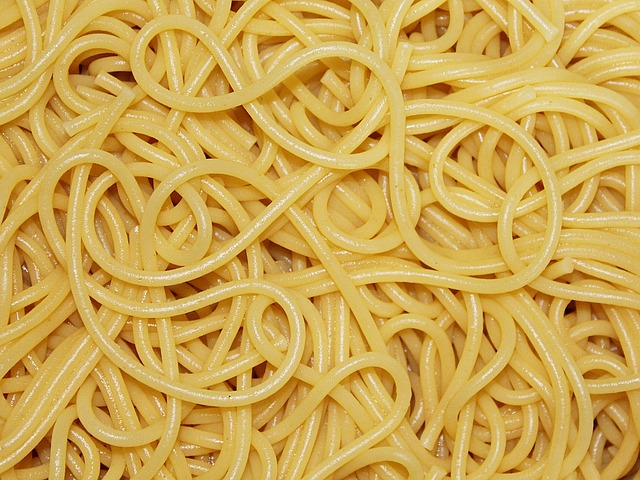
\includegraphics[width=.7\linewidth]{espaguetis}
\end{center}
\caption{Un plato de espaguetis sin estructurar}
\label{fig_pro}
\end{figure}

% Utilice «citet» para integrar el nombre del autor en el
% texto. Para referencias aisladas, «citep».

Durante la década de los sesenta, con el asentamiento del
concepto de la \emph{programación estructurada}, se fue
forjando un rechazo al recurso a esa intrucción de los
lenguajes de programación de alto nivel. En su célebre
carta, \citet{1968_Dijkstra} se declara convencido de que
«the go to statement should be abolished from all
  “higher level” programming languages (i.e. everything
  except—perhaps—plain machine code)». Ese \emph{perhaps}
parecía estar pidiendo innovaciones radicales en la
aquitectura de procesadores.

La propuesta de privación del recurso a los «gotos» no gozó
del asentimiento general: «Dijkstra once told me that he
actually received “a torrent of abusive letters” after
publication of his article» \citep[p. 265]{1974_Knuth}.

Sin embargo, a pesar de lo contundente de algunas
expresiones de la carta, no debería interpretarse esta,
seguramente, como una condena absoluta sobre los saltos
(\citet{1974_Knuth} reproduce estas palabras de Dijkstra:
«please don’t fall into the trap of believing that I am
terribly dogmatical about»), ni menos aún deducir que la
eliminación de los «gotos» es la fórmula mágica para lograr
un programa bien estructurado.

Knuth planteaba como objetivo la definición de uno o varios
juegos de estructuras, como el manejo de excepciones, para
ponerlas a disposición del programador. Auguraba un lenguaje
de programación consensuado para el año 1984: «Will
\textsc{Utopia 84} or, perhaps we should call it
\textsc{Newspeak}, contain {\bf go to} statements?».

Parece escéptico sobre su desaparición completa:
«... several languages have appeared in which the designers
proudly announced that they have abolished the \textbf{go
  to} statement. [...] which originally replaced \textbf{go
  to’s} by eight so-called “escape” statements. And the
eight weren’t even enough; the authors wrote, “Our mistake
was in assuming that there is no need for a label once the
\textbf{go to} is removed,” and they later [...] added a new
statement “\textbf{leave} $\langle$label$\rangle$
\textbf{with} $\langle$expression$\rangle$” which goes to
the place \emph{after} the statement identified by the
$\langle$label$\rangle$. Other \textbf{go to}-less languages
[...] and language designers still feel the need for some
euphemism that “goes to” without saying \textbf{go to}».

Añade: «... we shouldn’t merely remove \textbf{go to}
statements because it’s the fashionable thing to do; the
presence or absence of \textbf{go to} statements is not
really the issue. [...] undisciplined \textbf{go to}
statements make program structure harder to perceive, and
they are ofter symptoms of a poor conceptual
formulation». But there has been far too much emphasis on
\textbf{go to} elimination instead of the really important
issues; people have a natural tendency to set up an easily
understood quantitative goal like the abolition of jumps,
instead of working directly for a qualitative goal like a
good program structure» \citep{1974_Knuth}.

Si la controversia polarizada es ingrediente imprescindible
para el interés general, la respuesta de \citet{1987_Rubin}
abanderó la posición favorable a los «gotos», achacándole
dos faltas a la carta de Dijkstra: ser académica y poco
convincente. Según él, la identificación entre programación
estructurada y sin «gotos» es lo que «has caused
incalculable harm to the field of programming, which has
lost an efficacious tool». Se queja de que «some people have
devised program complexity metrics penalizing \textbf{GOTOs}
so heavily that any program with a \textbf{GOTO} is
\emph{ipso facto} rated more complex than even the clumsiest
\textbf{GOTO}-less program».

Rubin propone, para mostrar la utilidad del «goto», la tarea
de programar la búsqueda de la primera fila no nula de una
matriz cuadrada.

% Reproduce un fragmento de código.
\codigo[commandchars=\\\{\}]{codigo_04c.c}{con}{7.5cm}
\hfill
\codigo{codigo_01b.c}{sin}{7.5cm}

% Añadiendo la opción «commandchars=\\\{\}», los caracteres
% \, { y } del archivo fuente se interpretan como código
% LaTeX y puede darse formato al código (manualmente). Hay
% que tener esto en cuenta cuando estos caracteres formen
% parte del código en sí.
%
% Sin esa opción, el fichero de reproduce tal cual.

Sin encontrar satisfactorias las contestaciones que se
opusieron a la carta de Rubin \citep{1987_Moore},
\citet{1987_Dijkstra} vuelve a la carga. Imbuido tal vez del
ánimo de la dispu\-ta, entra a degüello, sin tolerarle a
Rubin una vacilación entre mayúsculas y minúsculas
siquiera. Rechaza, por ejempo, el uso de las construcciones
{\tt and} (y {\tt or}) condicionales, como las que aparecen
en la versión «sin».

Dijkstra está a otros menesteres y no le duelen prendas en
añadir variables: «a competent professional programmer [...]
should not waste his time in pointing out that the boolean
variable \texttt{d} is superfluous».

\begin{center}
% Puede pasar parámetros al comando «VerbatimInput» del
% paquete «fancyvrb». Por ejemplo:
\codigo[numbers=none,frame=single]{codigo_05b.py}{}{11.5cm}
\end{center}

En esta memoria procuraremos esclarecer el siguiente problema:

% Un recuadro sombreado:
\begin{tcolorbox}
\lipsum[11]
\end{tcolorbox}

\end{comment}
%%%%%%%%%%%%%%%%%%%%%%%%%%%%%%%%%%%%%%%%%%%%%%%%%%%%%%%%%%%%%%%%%%%%%%%%%%%%%%%%%%%%%%%%%%%%%%%%%%%%%%%%%%%%%%%%%%%%%%%%%%%%%%%%%%%%%%%%%%%%%%%%%%%%%%%%%%%%%%%%%%%%%%%%%%%%%%%%%%%%%%%%%%%%%%%%%%%%%%%%%%%%%%%%%%%%%%%%%%%%%%%%%%%%%%%%%%%%%%%%%%%%%%%%%%%%%%%%%%%%%%%%%%%%%%%%%%%%%%%%%%%%%%%%%%%%%%%%%%%%%%%%%%%%%%%%%%%%%%%%%%%%%%%%%%%%%%%%%%%%%%%%%%%%%%%%%%%%%%%%%%%%%%%%%%%%%%%%%%%%%%%%%%%%%%%%%%%%%%%%%%%%%%%%%%%%%%%%%%%%%%%%%%%%%%%%%%%%%%%%%%%%%%%%%%%%%%%%%%%%%%%%%%%%%%%%%%%%%%%%%%%%%%%%%%%%%%%%%%%%%%%%
% Historia , problema y resultados.


%\begin{tcolorbox}
%Hola Mundo
%\end{tcolorbox}


%Dejar claro que cap1 y cap2 es una recopilacion de resultados no propios de cara a desarrollar el trabajo

A general problem is to estimate a quantity from an object, relaying only in a finite number of samples and the method used to acquire them.
%Texto de introducción sobre el uso de la estereología actualmente
When it comes to object sampling, Stereology is the quintessential science since it makes it able to estimate quantitative properties of spacial objects. According to \cite{CO.IAS.17.Hist.pdf}, ``Stereology is the science of geometric sampling'' whose applications extend to disciplines such as biology and materials science.\\

In traditional sampling on discrete populations, sampling units had to be accessible to observation. However, the target object in geometric sampling is a subset of space and the sample is obtained via the intersection between the object and what's called a \textit{test probe}. A \textit{test probe} is basically a regular arrangement of test points, lines, planes, or slabs whose size and shape are known and has some sort of randomness mechanism relative to the object (see \cite{CO.IAS.17.Hist.pdf}).\\

%Domingo
There is another area of research which has been popular for its application to sampling: Quasi-Monte-Carlo algorithms. Among other differences, it can be said that 
Stereology has traditionally focus on estimations using a small number of samples, whereas Quasi-Monte-Carlo algorithms study methods with large number of samples and deterministic error bounds. 
The goal of this bachelor thesis is to show common areas of interest and explore the applicability of sampling strategies in well-known estimators used in Stereology. Our findings show that these new estimators are competitive candidates and their performance seem to correlate with geometric properties of the object. These observations open new directions on how to tailor estimators for specific problems.\\
%DOMINGO

%Domingo: Dependiendo del tiempo que tengamos, quizás deberiamos poner algo de la estructura del documento.

This document is written with the aim to be accessible to all people with a degree in mathematics, trying to hint the deep ideas behind the proofs. Although this work tries to be self-contained, some results and concepts like dimension, measure, etc. are not formally defined inside the document and we operate with them in an intuitive fashion.\\

The structure of the thesis is the following. Chapter 1 is devoted to give an ample introduction to Stereology and its fundamentals onto the estimators that will be used in the thesis. Chapter 2 recalls the theory of continuous probability and Hilbert spaces of functions, leading towards the Quasi-Monte Carlo integration method and optimal point sets for its use. Chapter 3 is focused on the evaluation and interpretation of computed results obtained with our python code for our new estimation methods. Finally, Chapter 4 end the thesis with some conclusions and future work.
\\[1cm]
\textit{Remark.} During Chapters \textbf{1} and \textbf{2}, a lot of history, theory and results have been gathered together in order to provide a simple understanding of the procedure and lead towards what we want to accomplish in this work. Therefore, the structure and information from these chapters will resemble to the ones from \cite{CO.IAS.17.Hist.pdf}, \cite{SterThAppl-2022-07-21.pdf}, \cite{Leobacher_Pillichshammer___2013___Introduction_to_Quasi_Montecarlo_Methods.pdf} and \cite{Hinrichs.pdf}.\\

\section{History}
%%%%%%%%%%%%%%%%%%%%%%%%%%% PROBLEMA: la historia está bastante copiada del pdf

%%%%%%%Historia
The underlying theory of Stereology is a blend of integral geometry, probability and statistics expected to be used in biomedical and material sciences. Since its development was focused on these two disciplines, Stereology can be divided in two branches depending on the application: 
%Domingo
\begin{itemize}
    \item \textit{Design based Stereology}: this area does not make any assumption about the data and the inference process is based on the randomness of the samples. It is more centered on biomedical applications, thus the object is assumed to be fixed and bounded and sampling is done with randomized test probes.
    \item \textit{Model based Stereology}: in this area there are some assumptions about the samples, specially some homogeneity in the object is assumed. It is more centered on material science applications where the object is huge, thus dealing with small portions of practically unbounded spacial structures and randomness being incorporated by means of a random set model (relies on model shapes, thereby usually leads to biased methods).
\end{itemize}
%DOMINGO.
Another distinction can be done regarding stereology that splits it into \textit{global stereology} and \textit{particle stereology}:
\begin{itemize}
    \item \textit{Global stereology}: In the design context it deals with total quantities (\textit{e.g.} total number, length, area, volume...). In the model context it deals with ratios (\textit{e.g.} relative volume).
    \item \textit{Particle stereology}: It deals with mean properties of individual particles (\textit{e.g.} mean volume).
\end{itemize}

Just as an introduction to this science, let's consider an equivalent problem to Buffon's needle problem, which is said to encapsulate the art and spirit of Stereology:\\
%Domingo
\begin{tcolorbox}
A needle of length $\ell$ is arbitrarily fixed inside a disk of diameter $h > \ell$ in the plane. A straight line in the same plane hits the disk at random. Calculate the probability that the straight line hits the needle\\
\end{tcolorbox}
%DOMINGO
Buffon's problem incorporates both a uniform random location of the center of the needle and a uniform random orientation (isotropic orientation) of the needle. We sketch the proof for the close formula for this probability using simple arguments. 
%Domingo: Aqui se hablaba de varias lineas pero en el  problema de buffon de una sola. He añadido una explicacion
An experimental approach would be to place ``random lines'' and count the proportion to estimate the probability.  
Now, if the number of random lines that hit the needle and the number of lines that miss the needle are known, then the ratio of those numbers would solve the problem. However, here it is necessary to use some sort of continuous geometric measure rather than traditional counting.\\

The following is an sketch with the main ideas needed to find the solution to Buffon's problem.
Let $L_1^2$ be a straight line used as a \textit{test probe}. This straight line can be defined with two coordinates $(p,\phi)$ in the plane, where $p \in (-\infty,\infty)$ is the distance of the line from a fixed origin $O$, and $\phi \in [0,\pi)$ is the orientation angle. Furthermore, the line can be associated with a density $\mathrm{d}L_1^2=\mathrm{d}p\mathrm{d}\phi$. Using this density, the total number of all straight lines hitting a convex set of boundary length $B$, is exactly $B$.\\
%DOMINGO (Quiza una referencia a la densidad y donde está el resultado con la página del libro de Luis)

%Domingo
For a needle of length $\ell$, the hitting measure (namely the measure of all the probes hitting the set) is $2\ell$. The reason is because the needle has to be regarded as a flattened convex set of perimeter $2\ell$. For the same reason, the hitting measure is $\pi h$ for a disk of diameter $h$. Therefore, the probability is $2\ell/(\pi h)$.\\
%DOMINGO


This result aroused controversy, %Domingo: Referencia? 
resulting on the appearance of paradoxes such as ``Bertrand's paradoxes''. A few years later it was discovered that measure densities had to be motion invariant, %Domingo: Referencia?  (Co.hist, está abajo)
that is, invariant with respect to translations and rotations, therefor making them independent of the reference frame.\\

All these events made integral geometry emerge as a mathematical discipline used to obtain motion invariant densities for geometric objects, thus establishing a foundation of geometrical probability. Some typical integral geometry results are the Crofton formulas, which relate intersections between two objects and their properties (number, length, area, volume...). %Domingo:REferencia (Co.Hist) y explica que son en una frase y porque son interesantes para nosotros (solo se usan para la explicación de como se obtiene un estimador en estereología)
For example, let $Y$ be a bounded planar curve  of finite length $B$. The measure of the number $I(Y\cap L_1^2)$ of intersections determined by all the motion invariant straight lines hitting the curve is 
\begin{equation} \label{eq2}
    \int_{Y}  I(Y\cap L_1^2)\,\mathrm{d}L_1^2 = 2B
\end{equation}
%Domingo: Me costo entender que tenia en este parrafo.
If $Y$ is the boundary of a convex set, then $I(Y\cap L_1^2)=2$, therefore the preceding formula yields the solution of Buffon's problem, noting the hitting measure is $B$.\\

%Domingo: He escrito esta frase, pero no sé que te parece
The minimal requirement to sample by intersecting with a probe is that we obtain information. For that,
Stereology also takes into account dimensional considerations in order to obtain the desired quantity. Depending on the dimension of the object and the probe, different procedures can be used and
%Domingo: he cambiado measures por parameters
different parameters have to be taken into account. To be more specific, for an object $Y$ hit by a probe $T$ in $\mathbb{R}^d$,
\begin{equation*}
    dim(Y\cap T) = dim(Y) + dim(T) - d
\end{equation*} 
holds up to a set of positions of zero measure. Since $dim(Y\cap T)\geq 0$, the following inequality must always hold,
\begin{equation}\label{eq1}
    dim(Y) + dim(T)\geq d.
\end{equation} 

%Domingo: Siempre que pongamos referencia a una formula, ponemos eqref
If equation \eqref{eq1} holds and either $dim(Y)=d$ or $dim(T)=d$, then relating $Y$ and $T$ by a Crofton formula is viable as long as $T$ has a fixed orientation relative to $Y$. On the other hand, if $dim(Y)<d$ and $dim(T)<d$, then the density of $T$ has to be motion invariant.\\

%Domingo: No sé si hace falta una frase para unir el parrafo anterior con este. (está en orden cronológico)
The next breakthrough in history was that Buffon's problem and the development of sampling and statistics in the 20th century inspired estimation problems. Furthermore, proper probability measures for random probes were defined, which was fundamental in the development of stereology. For instance, the probability element associated with a test line hitting a disk is $$ \mathbb{P}(\mathrm{d}p,\mathrm{d}\phi) = \frac{\mathrm{d}p\mathrm{d}\phi}{h\pi}, \hspace{2mm} p\in[-h/2,h/2], \hspace{2mm} \phi \in [0,\pi), $$
namely the motion invariant density normalized by the measure of all test lines hitting the disk. This probability element implies that $\phi \in [0,\pi)$ is \textit{uniform random} (UR), that is, \textit{isotropic random} (IR) in the unit semicircle, whereas $p \in [-h/2,h/2]$ is independent and UR. Therefore, the test line is said to be \textit{isotropic uniform random} (IUR) hitting the disk.\\

%Domingo: No es tanto un ejemplo como una aplicacion a un problema. Hay que leerse este parrafo.
To show an application of the formula in equation \eqref{eq1} to an estimation problem, suppose $Y$ is a planar curve with unknown length $B$ contained in a disk of diameter $h$.  
We suppose that the curve is not possible to manipulate (straighten the curve, cut into pieces, etc) and it is necessary to estimate the parameter $B$.
In order to do that, we design the following sampling experiment or estimator.
The sampling experiment consists of a disk being hit by a IUR test line $L_1^2$. Considering equation \eqref{eq2}, since $I(Y\cap L_1^2)$ is an integer valued random variable, its expectation (mean value) is $$ \mathbb{E}[I(Y\cap L_1^2)] = \int  I(Y\cap L_1^2)\,\mathbb{P}(dp,d\phi) = \frac{2B}{h\pi}. $$
Therefore, $\widehat{B}=\frac{h\pi}{2} \cdot I(Y\cap L_1^2)$ is an \textit{unbiased estimator} (UE) of $B$.\\

%Domingo: He cambiado algo
On one hand, the mean of different unbiased estimations taken at random and independently can be used to approximate the length better.
On the other hand, one inconvenience of the following estimator is that some of those estimations could give wrong results, e.g. certain estimations can be zero if the test line misses the curve, which results on time and effort spent uselessly. 
%Domingo: He tenido que añadir que es systematic sampling and 
In practice, \textit{estimators} which sample in a strategic way, v.g. adding more test lines, is more convenient and generally more efficient than independent sampling because estimations are rarely zero and variances tend to be significantly lower (see \cite{CO.IAS.17.Hist.pdf}).\\

These gives two basic strategies for sampling:
\begin{itemize}
    \item Random sampling: which estimates the measures using different results obtained for random test probes.
    \item Systematic sampling:  which estimates the measures using specific test probes that may get better results. This usually implies some kind of dependence between samples.
\end{itemize}
%%%%%%%%%%%%%%%%%%%%%%%%%%%%%%%%%%%%%%%%%%%%%%%
\section{Estimation Problems}
%%%%%%%%%%% Buffon y conteo
Now that some of the basic concepts and ideas about stereology have been introduced, lets focus on the estimation problems that will be studied in this work.\\
\textbf{Notation}: 
Through the rest of the thesis, we use the following conventions,
\begin{enumerate}
    \item $Y$ will denote a compact set with $dim(Y)=q$ and \textit{q}-measure $\gamma(Y)$. For example, if $Y\subset \mathbb{R}^3$, then $\gamma(Y)$ may represent number of subsets, curve length, surface area or volume, depending on whether $q=0,1,2,3$ respectively.
    \item $L_r\equiv L_r^d, \hspace{2mm} r=0,1,...,d$ will denote an \textit{r}-plane in $\mathbb{R}^d$, for instance, a test point, line, plane or slab according to whether $r=0,1,2,3$ respectively.
    \item $\alpha(X)$ will denote the geometric measure of a compact set $X$, thus $\alpha(\emptyset)=0$. For example, if $Y\subset \mathbb{R}^3$, then $\alpha(Y\cap L_r)$ will represent number, length, area or volume, depending on whether $q+r-d=0,1,2,3$, respectively.
    \item The idea behind this work can be applied to most or all of the different estimation problems. Here we test its performance in two of them.
\end{enumerate}

\subsection{Test System of Quadrats}
%Domingo :  Maybe to add a phrase about what is a test quadrat of area. Maybe a graph.
Suppose $Y=\{ y_1,y_2,...,y_N \}\subset D \subset \mathbb{R}^2$ is a finite set of $N$ disjoint point particles where $y_i$ denotes the \textit{i}-th point particle and $D$ is a reference disk of diameter $H$. Consider $T_2^2(x,\omega)$, a test quadrat (square) of area $a$ and random fixed orientation $\omega \in [0,2\pi)$ that's free to move parallel to itself with translation invariant density $dT_2^2(x,\omega)=dx$. We have
\begin{multline} \label{eq3}
    \int_{\mathbb{R}^2}  N(Y\cap T_2^2(x,\omega))\,\mathrm{d}x = \int_{\mathbb{R}^2} \sum_{i=1}^N 1_{T_2^2(x,\omega)}(y_i),dx = \int_{\mathbb{R}^2} \sum_{i=1}^N 1_{T_2^2(0,\omega)}(y_i-x),dx \\ = \sum_{i=1}^N \int_{\mathbb{R}^2}  1_{T_2^2(0,\omega)}(y_i-x),dx = Na 
\end{multline}

The probability element for a quadrat with fixed orientation $T_2^2(x)$ hitting a disk $D$ is
\begin{equation*}
    \mathbb{P}(dx)=\frac{dx}{A(D_{\oplus})}, \hspace{2mm} x\in D_{\oplus}.
\end{equation*}
where $A(D_{\oplus})$ is the area of the geometric loci of the AP as the test probe hits D. Therefore, the number of point particles is
\begin{equation*}
    N=\frac{A(D_{\oplus})}{a}\cdot\mathbb{E}(Q(x))
\end{equation*}
where $Q(x)$ is the number of point particles captured by the quadrat. Similar results can be obtained for $\mathbb{R}^d$.\\

Since the quadrat's orientation is fixed, it is usually called a \textit{FUR quadrat} (Fixed Uniform Random). Let's consider a FUR quadrat $T_0 \equiv T_2^2(0,\omega) \subset J_0 \subset \mathbb{R}^2$ of area $a_0 > 0$ and fixed orientation $\omega \in \mathbb{S}$ where $T_0$ is what's called a \textit{fundamental probe} contained in a \textit{fundamental tile} $J_0$ of the test system. A \textit{FUR test system of quadrats} can be defined as 
\begin{equation*}
    \Lambda_x := \{ T_2^2(x+t_k,\omega), k\in \mathbb{Z} \}, \hspace{2mm} x \sim UR(J_0)
\end{equation*}
% Domingo: Aquí haria falta una referencia a la página (229 pdf).
Considering equation \eqref{eq3} and Santaló's formula for FUR test systems with bounded fundamental test probes $T_0\subset J_0\subset \mathbb{R}^d$,
\begin{equation*}
    \gamma(Y)\nu(T_0)=\int_{J_0}  \alpha(Y\cap \Lambda_x)\,\mathrm{d}x
\end{equation*}
where $\gamma(Y)$ is the target measure, $\nu(T_0)$ is the known measure for the fundamental probe and $\alpha(Y\cap \Lambda_x)$ is the geometric measure of $Y\cap \Lambda_x$, we have
\begin{equation*}
    \gamma(Y)\cdot a_0 = \int_{J_0}  \alpha(Y\cap \Lambda_x)\,\mathrm{d}x = a\cdot \mathbb{E}[\alpha(Y\cap \Lambda_x)]
\end{equation*}
where $a\geq a_0$ is the area of $J_0$. Therefore, the basic identity for a FUR test system of quadrats is
\begin{equation} \label{conteo}
    \gamma(Y)=\frac{a}{a_0}\cdot \mathbb{E}[\alpha(Y\cap \Lambda_x)]
\end{equation}
where $\gamma = N \text{ (number)},B \text{ (length)},A \text{ (area)}$ depending on whether $dim(Y)=0,1,2$ respectively (\cite{SterThAppl-2022-07-21.pdf}).\\

In this work, $Y$ will be a set of point particles representing people in different photos. This means that $dim(Y)=0$, thus the identity that will be used reads
\begin{equation} \label{Conteo_usada}
    N =\frac{a}{a_0}\cdot \mathbb{E}[N(Y\cap \Lambda_x)]
\end{equation}

Later in this work we will use the aforementioned identity to estimate the amount of points present in photos and compare the efficiency of the usual programming methods with a new method that will be explained.\\

\subsection{Buffon-Steinhaus Test System}

Suppose $Y\subset \mathbb{R}^2$ is a curve  of finite length $B>0$. The \textit{Buffon test system} consists of IUR parallel test lines separated by a constant distance $T>0$, that is,
\begin{equation*}
    \Lambda_{x,\omega} := \{ L_1^2(x+kT,\omega), \hspace{2mm} k\in \mathbb{Z} \}, \hspace{2mm} x\sim UR[0,T], \hspace{2mm} \omega \sim IR[0,\pi].
\end{equation*}

In this case, a straight line $L_1^2(0,\omega)$ is the fundamental probe, and the fundamental tile for the auxiliary test system of points on an axis normal to the test lines is the segment $J_0=[0,T)$. Thus, the joint probability element is
\begin{equation*}
    \mathbb{P}(\mathrm{d}x,\mathrm{d}\omega)=\frac{\mathrm{d}x}{T}\cdot \frac{\mathrm{d}\omega}{\pi}, \hspace{2mm} x\in [0,T), \hspace{2mm} \omega \in [0,\pi)
\end{equation*}

Now, considering Santaló's formula for an IUR test system of unbounded \textit{r}-planes in $\mathbb{R}^d$,
\begin{equation*}
    c_1\cdot \gamma(Y) = \int_{G_{r,d-r}}\,\mathrm{d}\omega \int_{J_0} \alpha(Y\cap \Lambda_{x,\omega})\,\mathrm{d}x,
\end{equation*}
where $G_{r,d-r}$ is \textit{the Grassmannian} (\textit{i.e.} the space of all non oriented \textit{r}-subspaces $L_{r[0]}^d\equiv L_r^d(0,\omega)$ acted upon by the group of rotations of $\mathbb{R}^d$), the corresponding identity reads
\begin{equation*}
    \gamma(Y) = \frac{c_{10}}{c_1}\cdot V(J_0)\cdot \mathbb{E}[\alpha(Y\cap \Lambda_{x,\omega})],
\end{equation*}
where $V(J_0)$ represents the 'volume' of $J_0$, $q=dim(Y)$,
\begin{equation*}
    \frac{c_{10}}{c_1} = \frac{O_q O_r}{O_d O_{q+r-d}},
\quad
\mathrm{ and }\ 
%Domingo: Correct this equation. I don't know if it is k or k+1 (62 pdf)
    O_k = \frac{2\pi^{(k+1)/2}}{\Gamma((k+1)/2)}, \hspace{2mm} k=0,1,...,d,
\end{equation*}
is the surface area of the \textit{k}-dimensional unit sphere $\mathbb{S}^k$.\\

With the aforementioned test system, $\gamma(Y)=B$, $c_{10}/c_1=\pi/2$ and $V(J_0)=T$. Therefore, the basic identity for the Buffon test system is
\begin{equation} \label{Buffon}
    B=\frac{\pi}{2}\cdot T \cdot \mathbb{E}[I(Y\cap \Lambda_{x,\omega})].
\end{equation}

In this work we will also use the \textit{Buffon-Steinhaus test system}, also called the \textit{square grid}. This system is the union of two perpendicular Buffon test systems, thus, the test length per unit area is doubled and $T$ should be replaced with $T/2$. Whereby, the basic identity for the Buffon-Steinhaus test system is
\begin{equation} \label{Buffon_Steinhaus}
    B = \frac{\pi}{4} \cdot T \cdot \mathbb{E}[I(Y\cap \Lambda_{x,\omega})].
\end{equation}

Alternatively, one may keep the test system fixed and the target set $Y\equiv Y(x,\omega)$ mobile, in which case
\begin{equation*}
    B = \frac{\pi}{4} \cdot T \cdot \mathbb{E}[I(Y(x,\omega) \cap \Lambda_{0,0})],
\end{equation*}
% Domingo: I rephrase this.
which gives the same estimator (\cite{SterThAppl-2022-07-21.pdf}).\\

%COMPROBAR SI ESTO CUADRA BIEN CON LO ANTERIOR
That being said, later in this work we will use the aforementioned identity to estimate the length of specific curves and compare the efficiency of the usual programming methods with the new method.\\


